\chapter{Aufbau}
\section{Elektrischer Aufbau}



%
\section{Mechanischer Aufbau}\label{sec:mechanischer_Aufbau}
	\subsection{St�ckliste}
	\begin{enumerate}
		\item Plexiglasrohr
		\item Plexiglasscheibe
		\item 4 M6 Schrauben
		\item 8 M6 Muttern
		\item 8 M6 Unterlagsscheiben
		\item Anschlussteil einen HT-Abwasserrohrs
		\item L�fter
		\item Abstandssensor
		\item Patex 2K Kleber
		\item Sekundenkleber
	\end{enumerate}
\subsection{Beschreibung}
Die Plexiglasscheibe dient als Basis des gesamten mechanischen Aufbaus (siehe Abb. \ref{fig:Aufbau_gesamt}). In ihrer Mitte befindet sich ein Loch durch welcher das HT-Rohr, bis zur Dichtungsverbreiterungs, genau durchpasst. Obwohl das HT-Rohr schon durch eine Presspassung in der Plexiglasscheibe h�lt wurde es zus�tzlich mit Zweikkomponentenkleber fixiert. In die vier Ecken der Scheibe wurde L�cher gebohrt, durch diese wurden die Schrauben gesteckt und mit den Mutter sowie den Unterlagsscheiben fixiert. Die Schrauben dienen Als F��e f�r den Aufbau. Dies hat fogende Vorteile:
\begin{itemize}
		\item Der L�fter liegt nicht dirkt auf dem Untergrund und kann somit Luft ansaugen.
		\item Der Aufbau steht stabil auf dem Untergrund.
		\item Durch die Verwendung von Schrauben kann ein unebener Untergrund ausgeglichen werden.
\end{itemize}

In die Verbreiterung des HT-Rohrs befindet sich normalerweise eine Gummidichtung. In unserem Fall kann dort aber der L�fter bequem eingeclipst werden. Auf dem L�fter wurde der Abstandssensor mit Sekundenkleber befestigt. Da der Sensor einen Steckanschluss hat und dieser im fertigen Aufbau nicht mehr erreicht werden kann, wurde dieser mit Litzen, am L�fter vorbei unten aus dem HT-Rohr gef�hrt. In das andere Ende des HT-Rohrs wird das Plexiglas Rohr gesteckt werden, dieses passt ebenfalls genau dort hinein und ist somit durch eine Presspassung fixiert (siehe Abb. \ref{fig:IMG_20160523_191318}).

\begin{figure}[!htb]
	\centering
	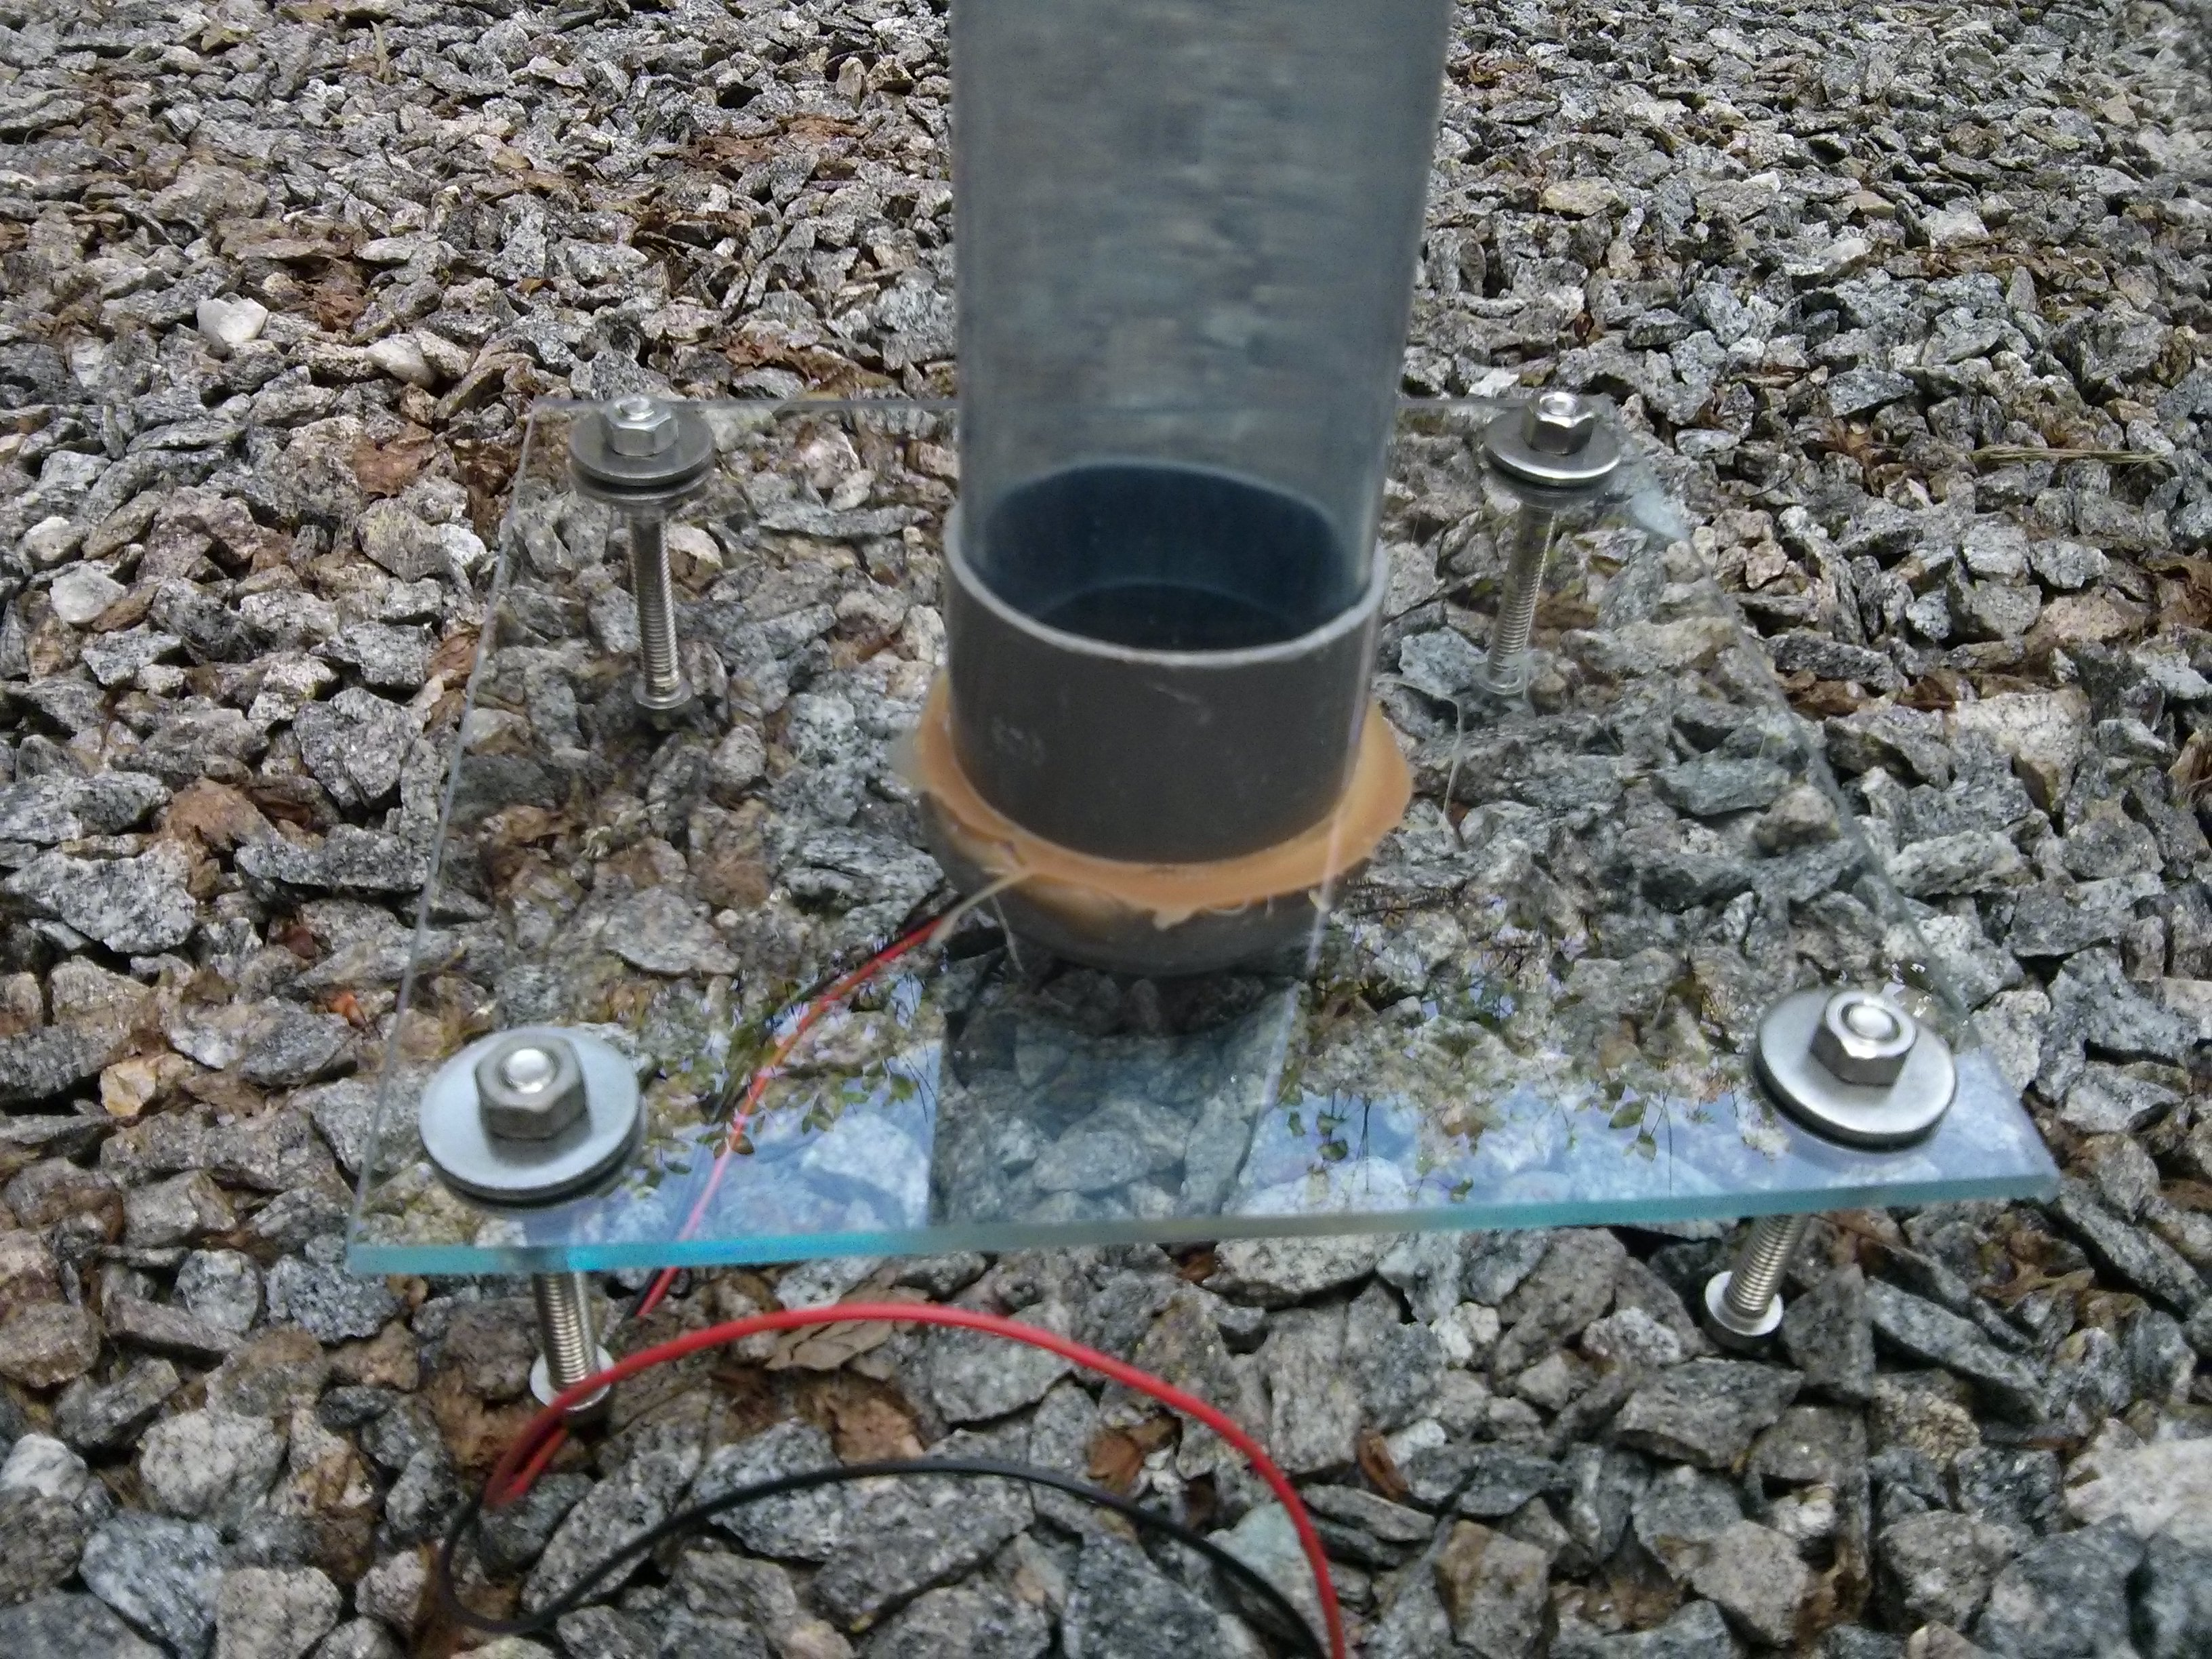
\includegraphics[width=0.8\linewidth]{./Bilder/IMG_20160517_152455}
	\label{fig:Aufbau_gesamt}
	\caption{Fertiger mechanischer Aufbau}
\end{figure}
\begin{figure}[!htb]
	\centering
	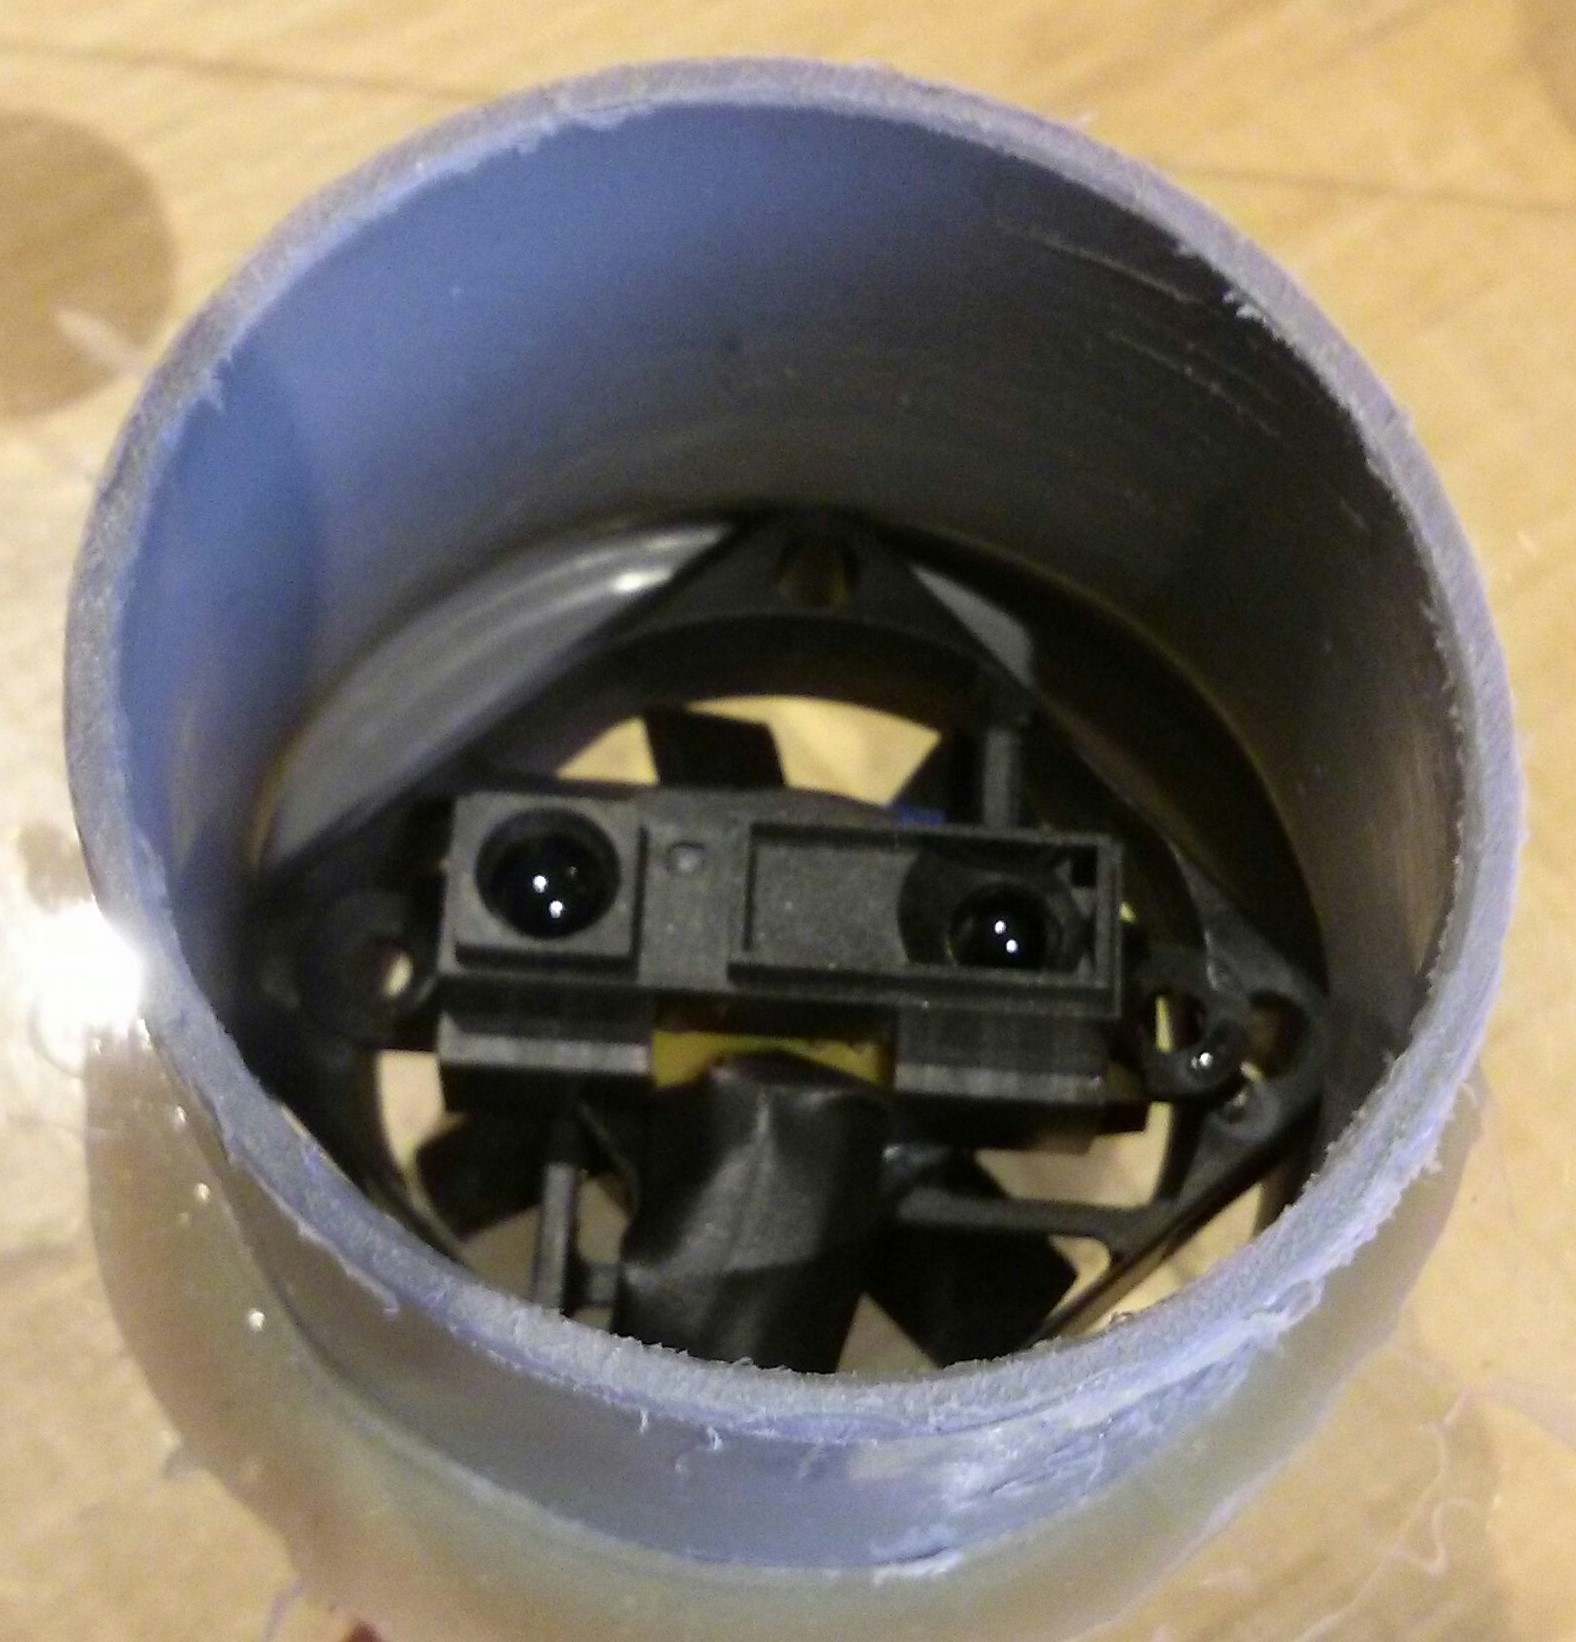
\includegraphics[width=0.6\linewidth]{./Bilder/Luefter_mit_Sensor_im_Rohr}
	\caption{L�fter mit Sensor im HT-Rohr}
	\label{fig:IMG_20160523_191318}
\end{figure}
%

\section{Elektrischer Aufbau}\label{sec:elAufbau}
%
\subsection{Die Schaltung}\label{ssc:schaltung}
%
Der Schaltplan wird auf Abb. \ref{fig:schaltplan} dargestellt.
Der Abstandssensor ist �ber die Steckverbindung J11 mit der Platine verbunden. Versorgt wird der Sensor mit einer Spannung von 5V, die �ber den USB Stecker J10 geliefert wird. Die Widerst�nde R1 bis R4 bilden zusammen mit dem Operationsverst�rker IC1 einen Differenzverst�rker, der die Spannung am Ausgang des Abstandssensors f�r das Mikrocontrollerboard entkoppelt.\\
Der Operationsverst�rker wird mit einer Spannung von 3,3V versorgt, die vom Mikrocontrollerboard �ber J1 geliefert wird. Der Ausgang des OPs am Pin 1 des IC1 ist mit dem AD-Wandler Eingang ADCA1 des Controllers verbunden, um das Messsignal zu digitalisieren.\\
Da der L�fter mit 5V betrieben wird und zu viel Strom ben�tigt, den der Mikrocontroller nicht liefern kann, wird er �ber einen Optokoppler betrieben. Der Mikrocontroller liefert ein PWM Signal am Ausgang EPWM1A an J6, das dann �ber den Vorwiderstand R5 den Optokoppler IC2 ansteuert. Am Ausgang des Optokopplers ist der L�fter �ber J12 angeschlossen.\\
\\
Die Ma�e der Platine sind gleich gro�, wie die das Mikrocontrollerboard, sodass es genau auf die Entkopplungsplatine aufgesetzt werden kann. �ber die Buchsen J1, J2, J5 und J6 werden die n�tigen Verbindungen zwischen der Entkopplungsplatine und dem Mikrocontrollerborad hergestellt und dienen gleichzeitig als mechanischen Halt, sodass zwischen Mikrocontrollerboard und der Entkopplungsplatine keine zus�tzlichen Schrauben oder �hnliches mehr notwendig sind.\\
\\
Das Mikrocontrollerboard wird �ber ein Mini USB Kabel sowohl mit Strom versorgt, als auch die Verbindung um den Controller zu programmieren, hergestellt. Die Entkopplungsplatine wird �ber ein USB A Stecker mit einer USB Spannungsquelle, wie zum Beispiel einem Ladeger�t, verbunden.
%
\begin{figure}[htb]
	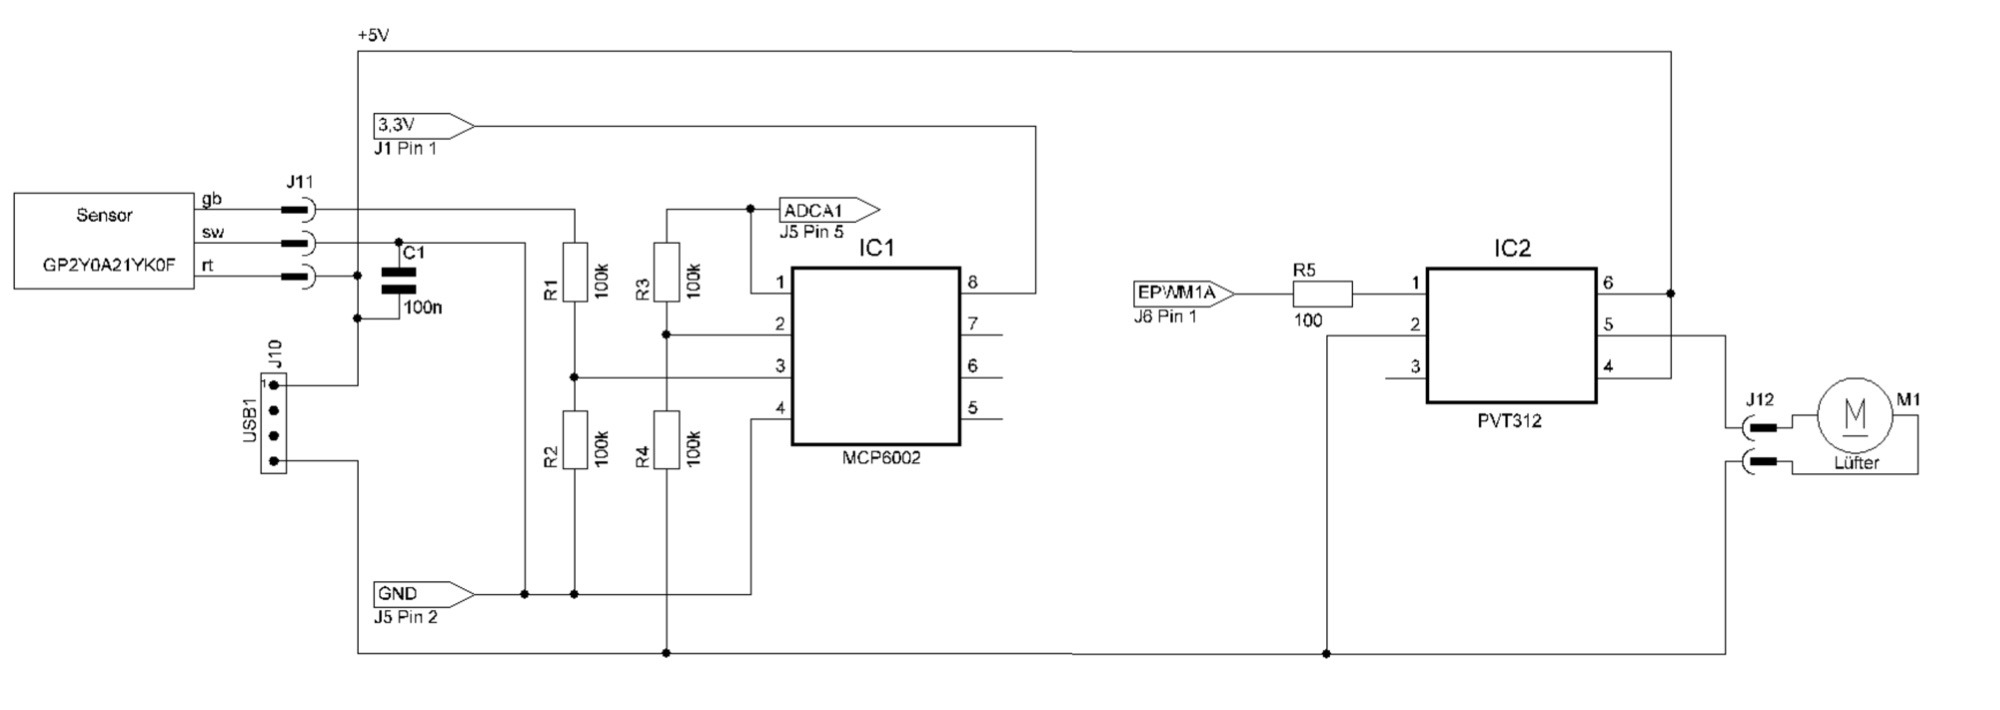
\includegraphics[width = \linewidth]{./Bilder/schaltplan}
	\caption{Schaltplan mit Pinout}
	\label{fig:schaltplan}
\end{figure}
\subsection{Das Layout}\label{ssc:layout}
%
Die Schaltung ist auf einer Lochrasterplatine realisiert und die Leiterbahnen mit Silberdraht gel�tet (siehe Abb. \ref{fig:layout}). Das Layout ist so gew�hlt, dass m�glichst wenige Kreuzungen entstehen um Br�cken auf der Best�ckungsseite zu vermeiden. Da von J1, J2 J5 und J6 nicht alle Pins ben�tigt werden, sind auch nur die n�tigsten Stiftleisten aufgel�tet. Die Lochrasterplatine mit Controller kann auf Abb. \ref{fig:platContr} betrachtet werden.

%
\begin{figure}[htb]
	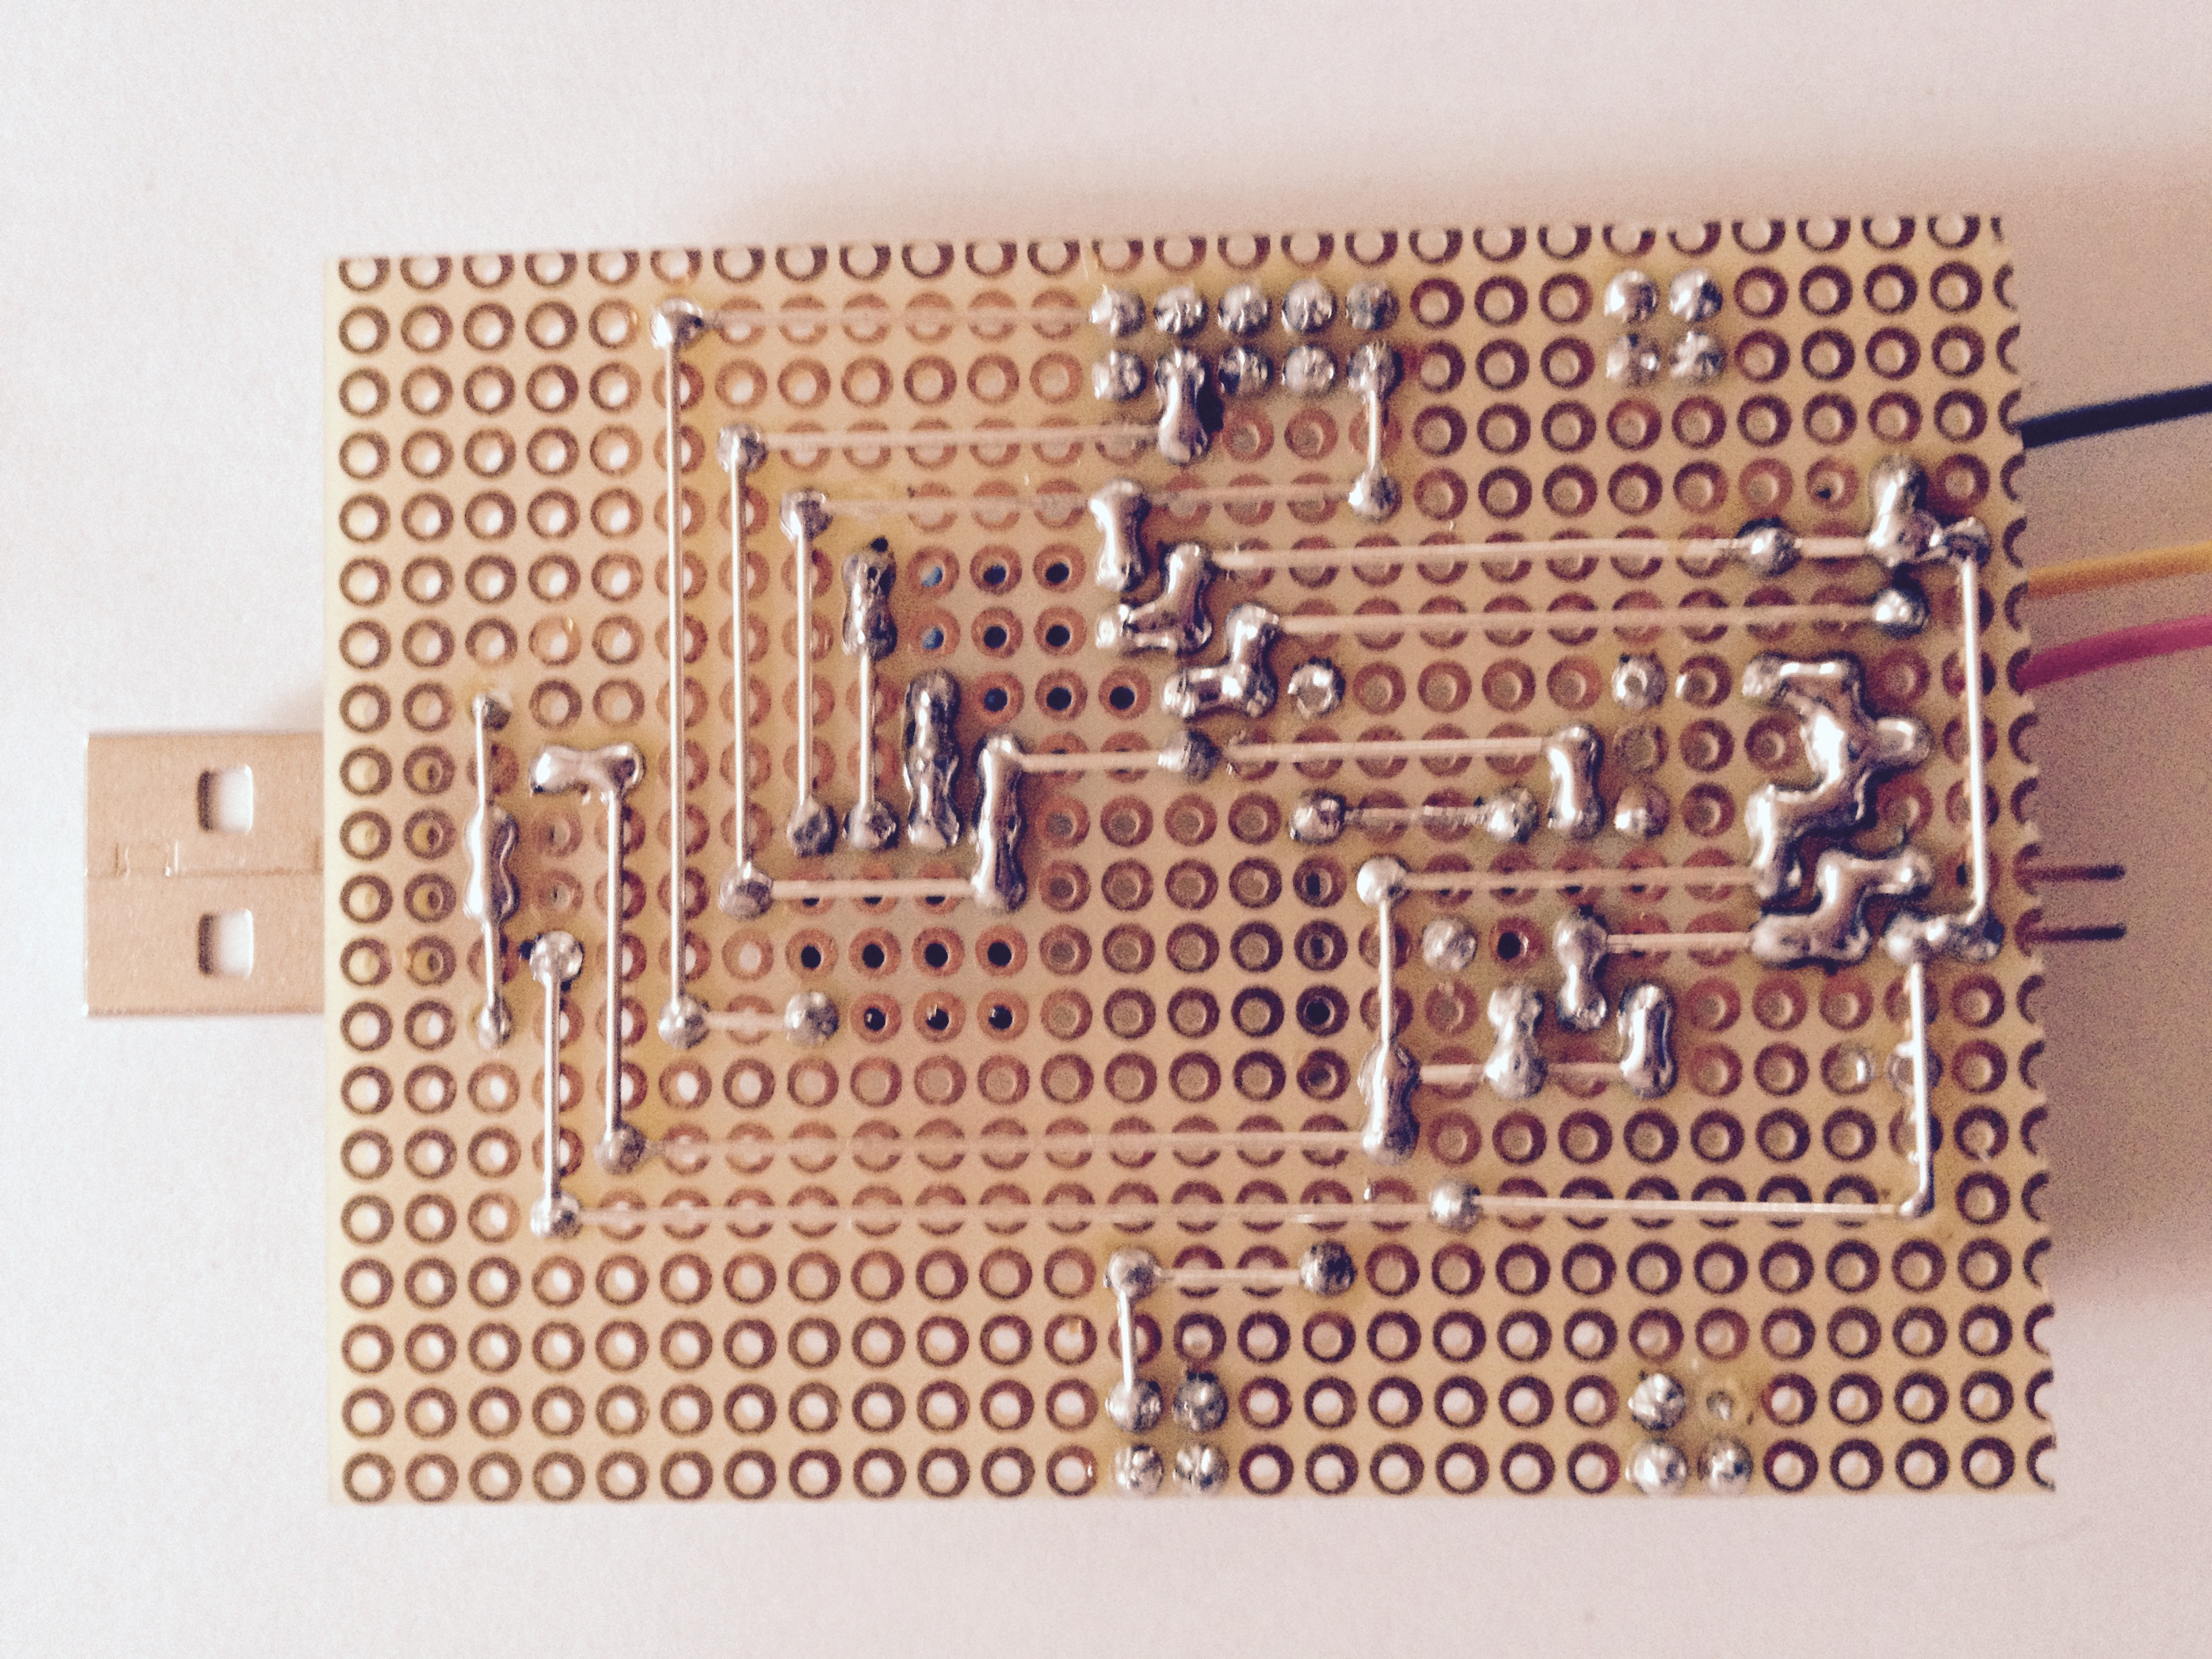
\includegraphics[width = 0.8\linewidth]{./Bilder/Layout}
	\caption{Lochrasterplatine R�ckseite}
	\label{fig:layout}
\end{figure}

\begin{figure}[htb]
	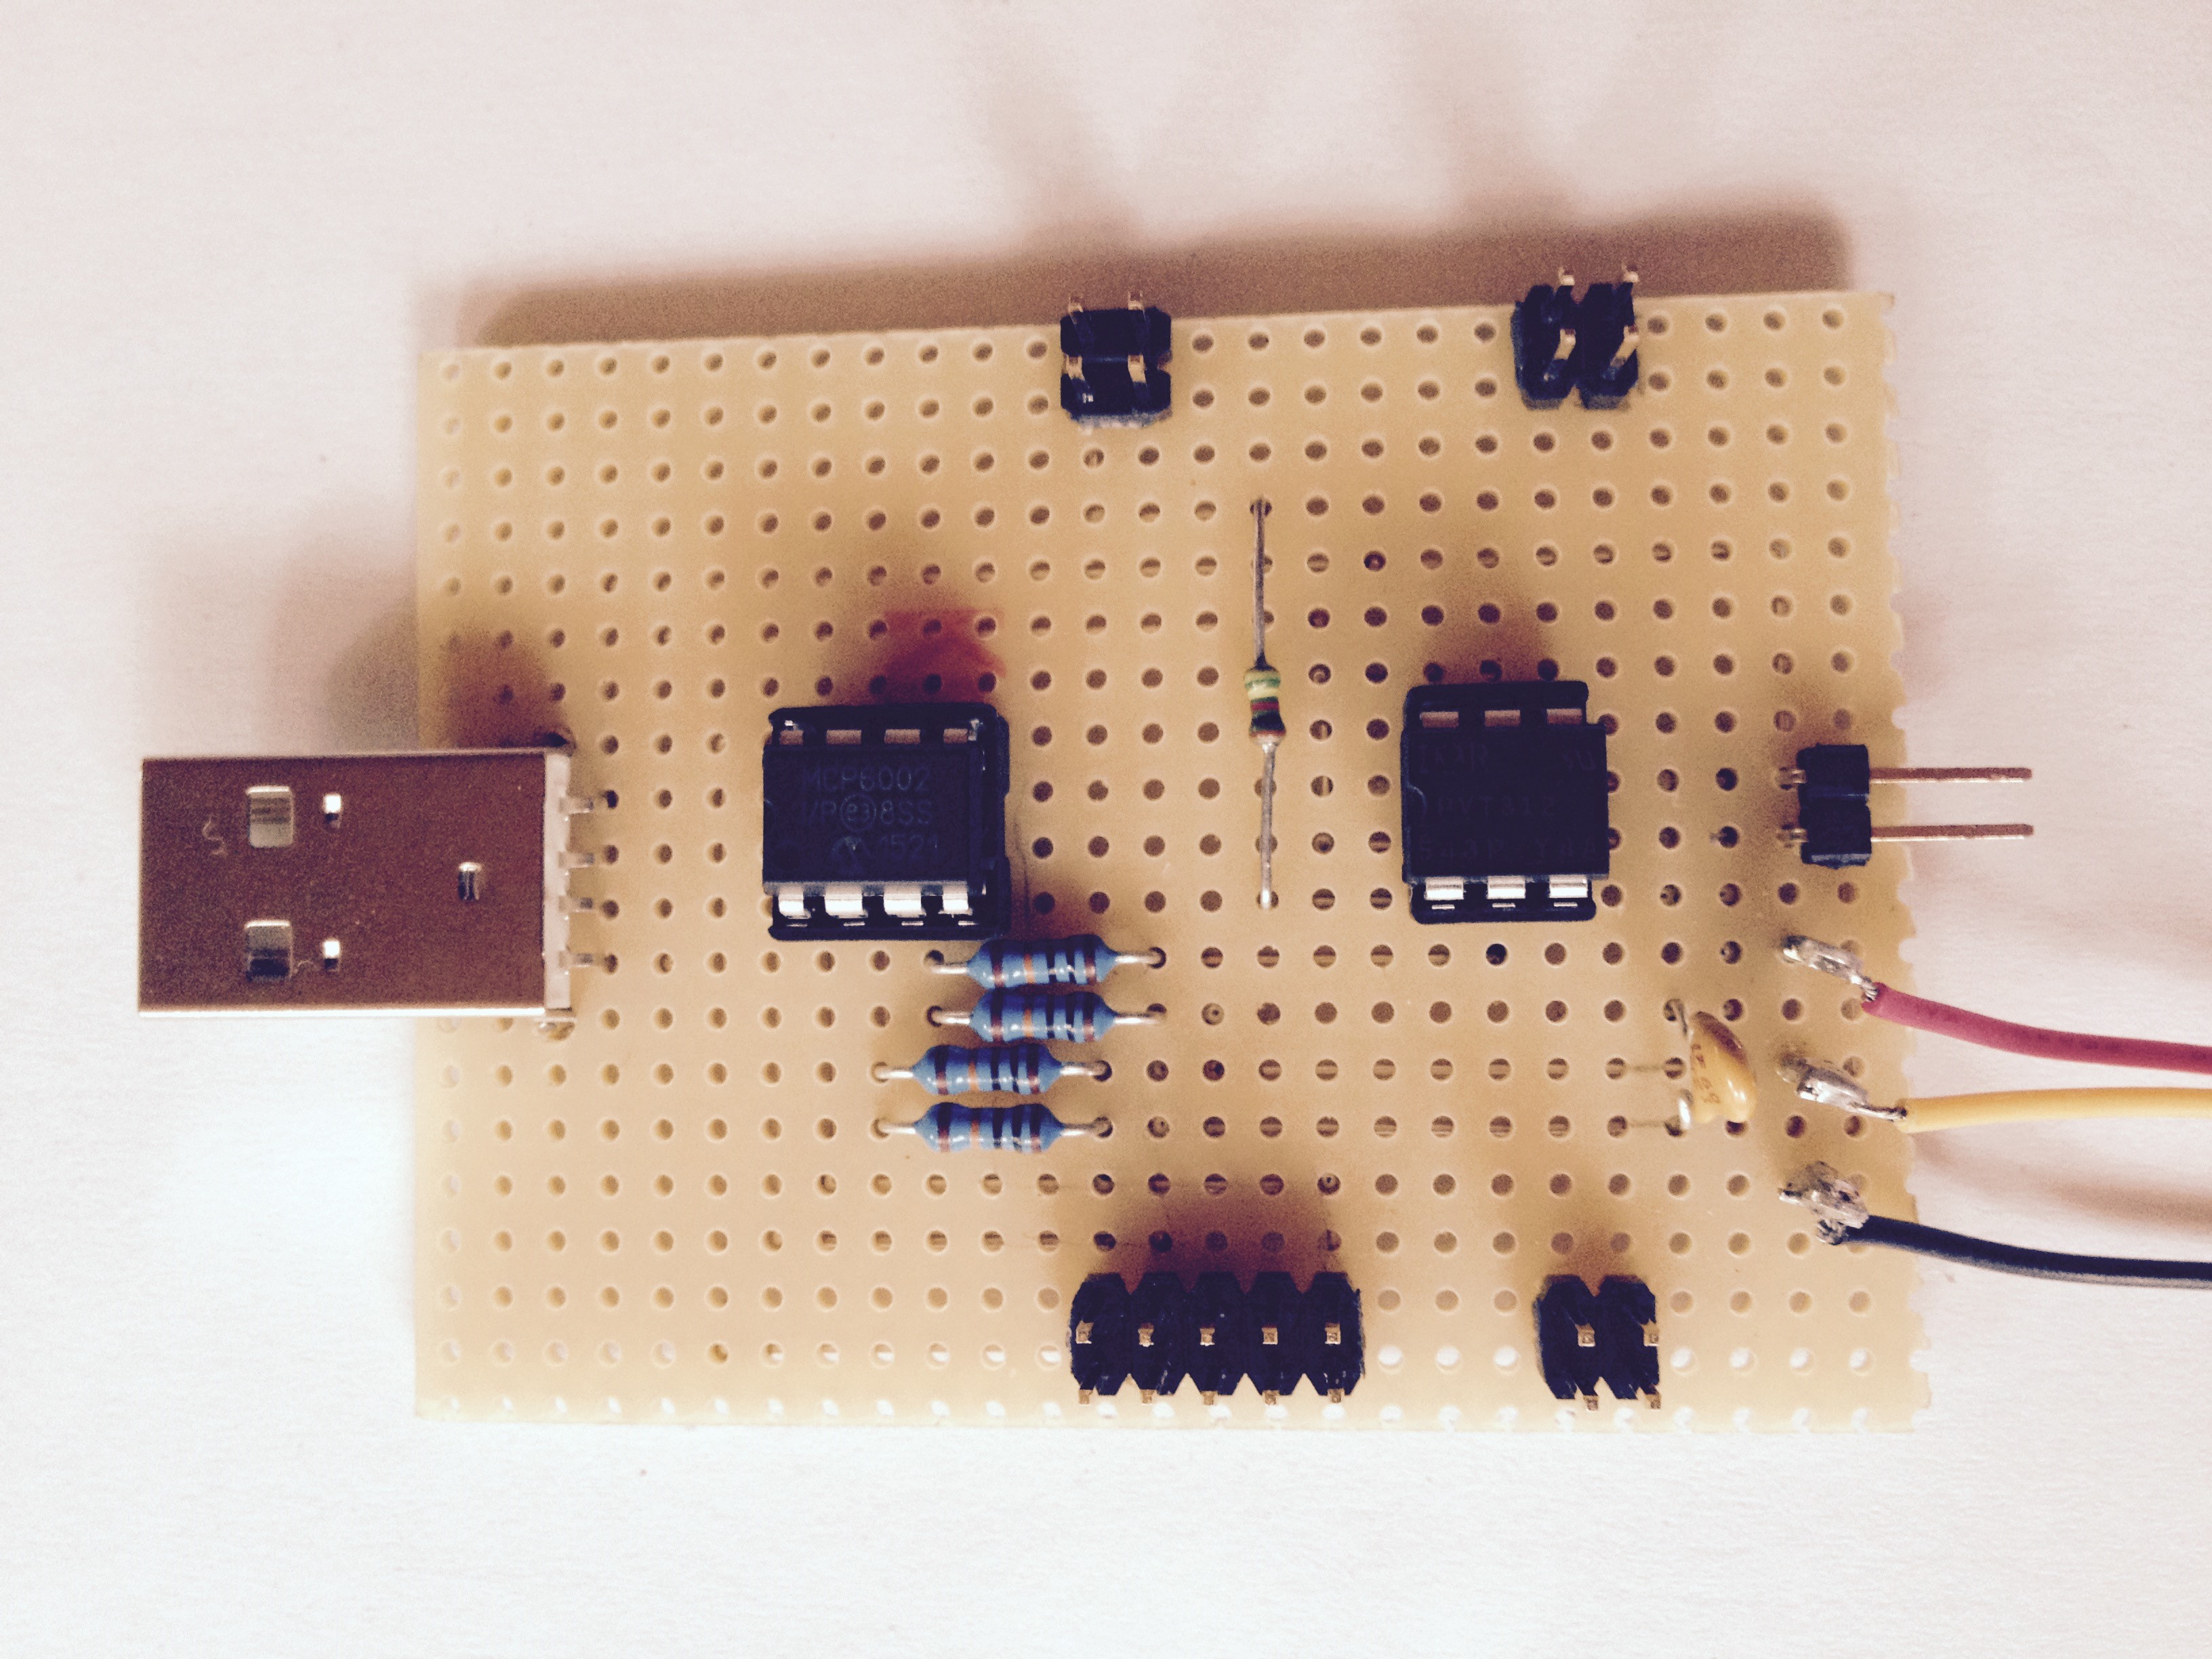
\includegraphics[width = 0.8\linewidth]{./Bilder/Bestueckung}
	\caption{Lochrasterplatine Best�ckungsseite}
	\label{fig:best�ckungsseite}
\end{figure}

\begin{figure}[htb]
	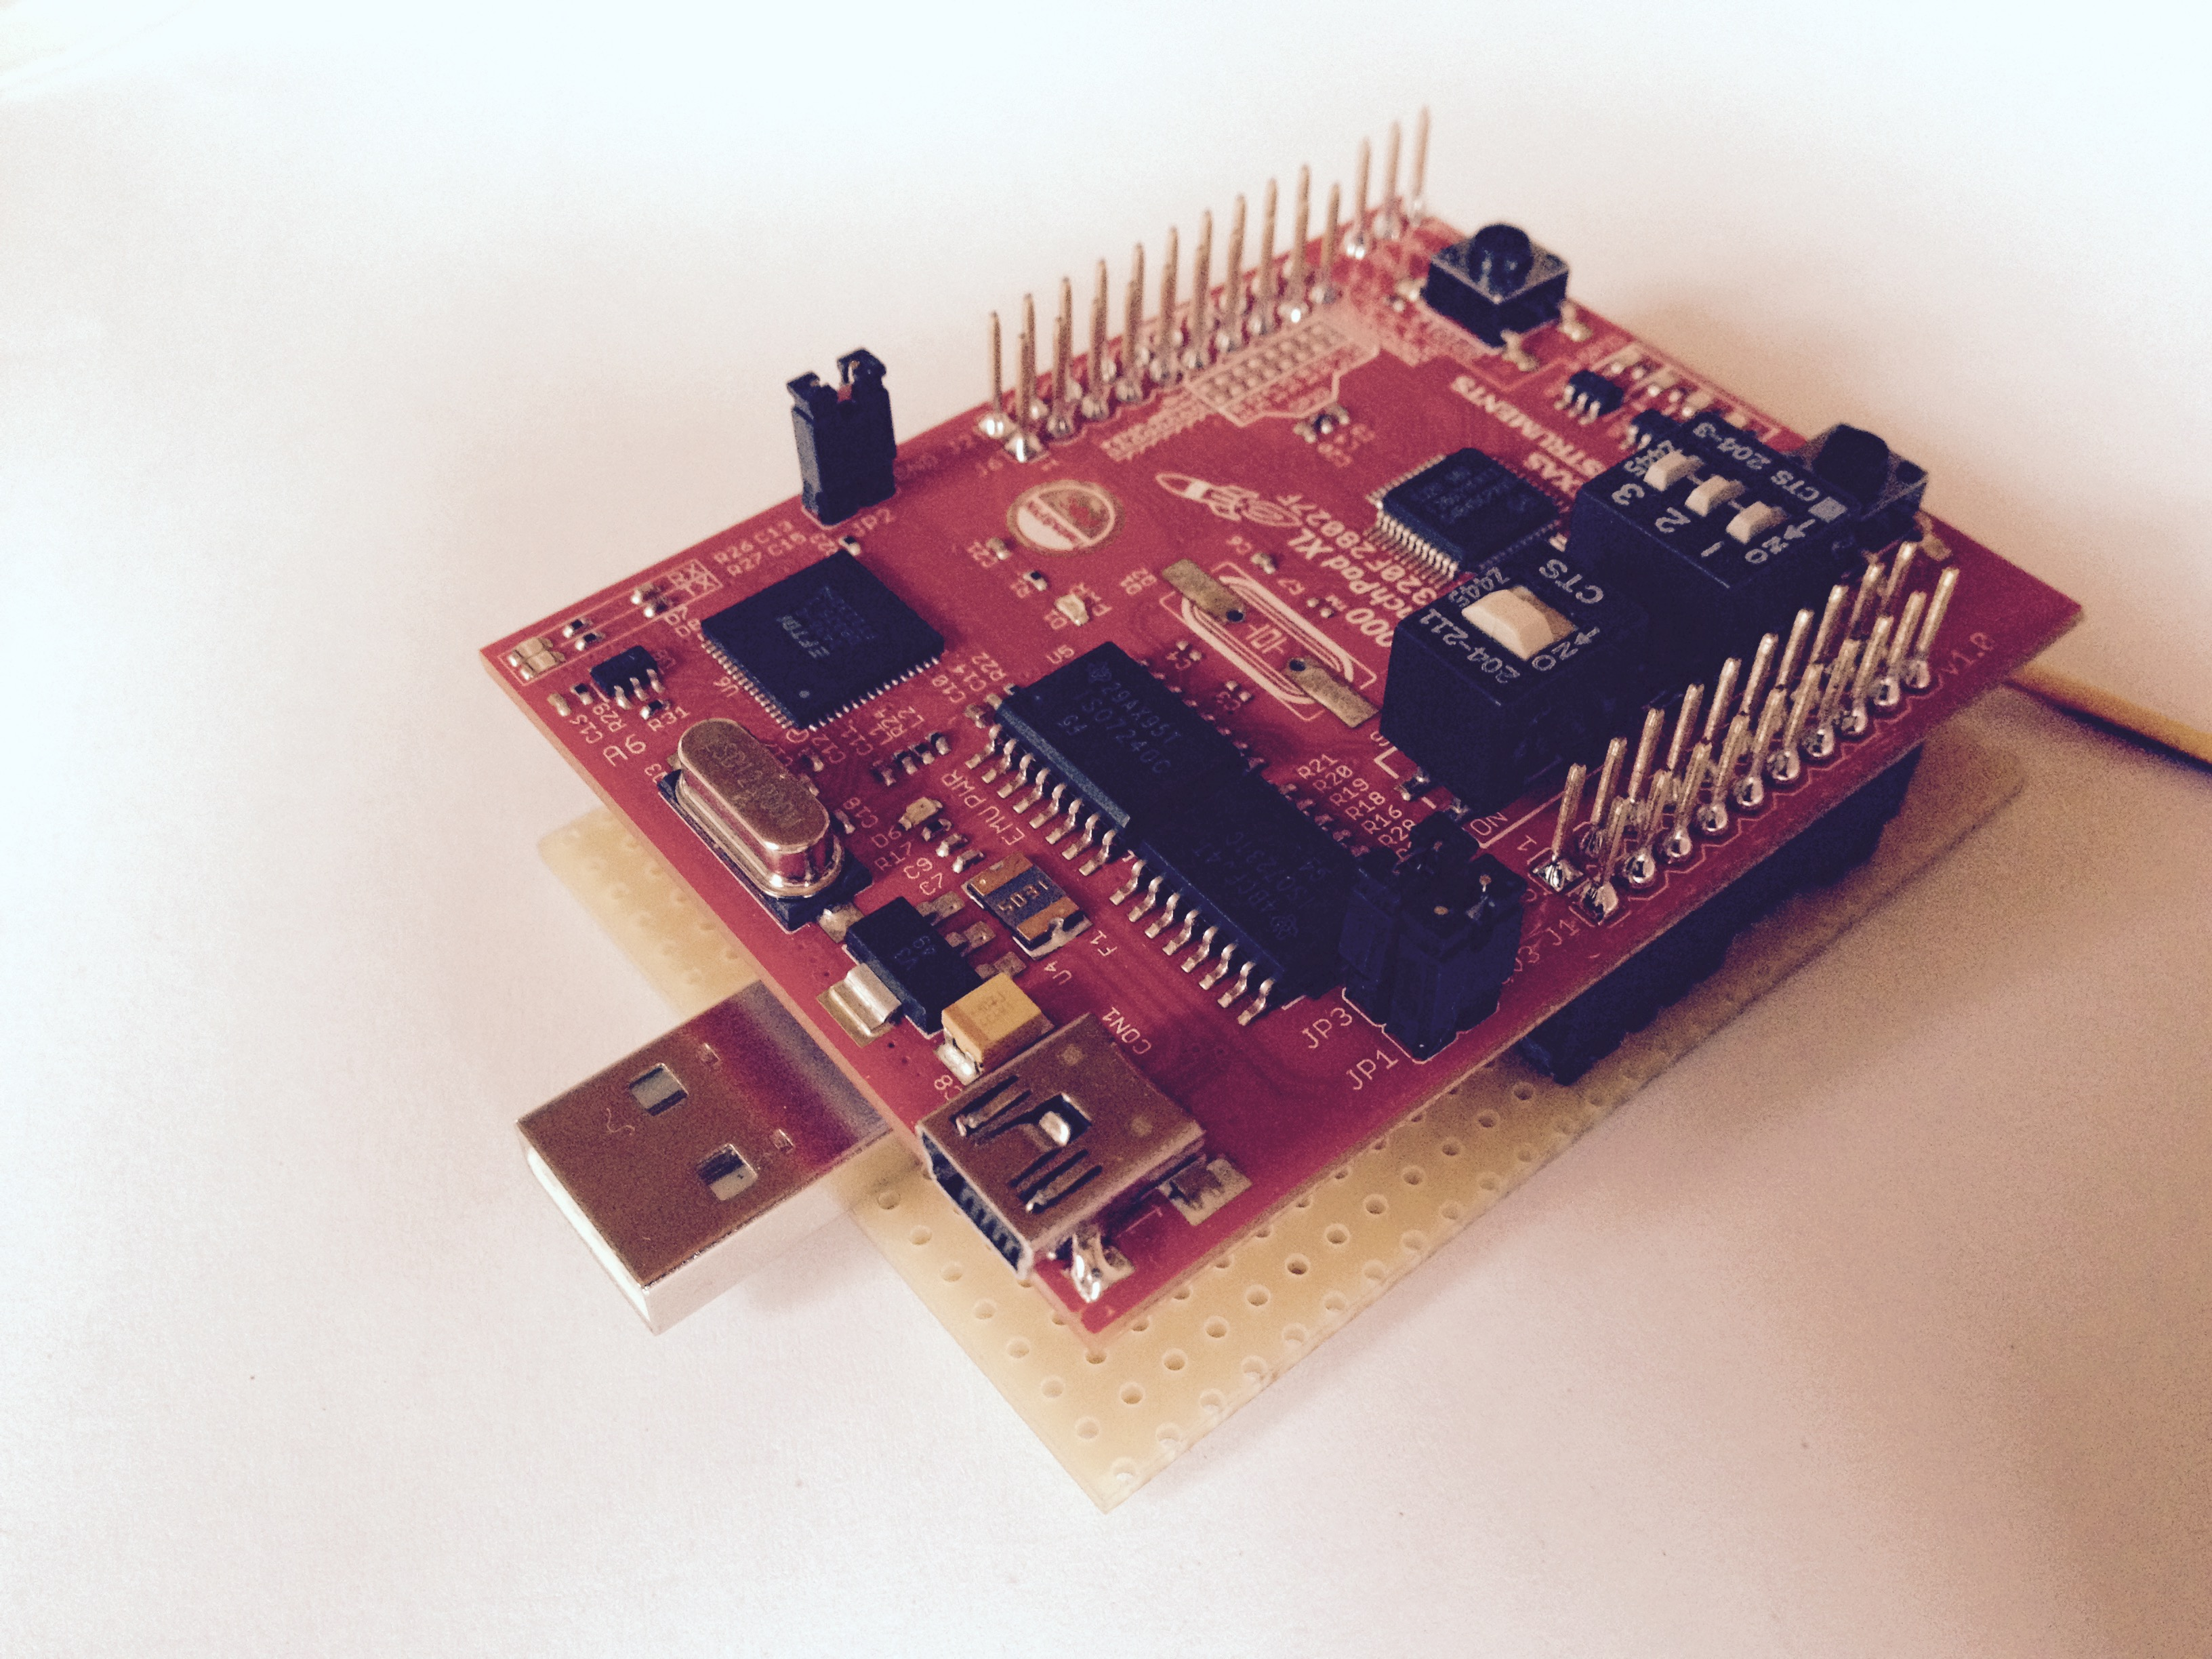
\includegraphics[width = \linewidth]{./Bilder/Platine_mit_Controller}
	\caption{Lochrasterplatine mit Controller}
		\label{fig:platContr}
\end{figure}